\documentclass[spanish,a4paper,10pt]{article}

\usepackage{latexsym,amsfonts,amssymb,amstext,amsthm,float,amsmath}
\usepackage[spanish]{babel}
\usepackage[latin1]{inputenc}
\usepackage[dvips]{epsfig}
\usepackage{doc}
\usepackage{graphicx}

%%%%%%%%%%%%%%%%%%%%%%%%%%%%%%%%%%%%%%%%%%%%%%%%%%%%%%%%%%%%%%%%%%%%%%
%123456789012345678901234567890123456789012345678901234567890123456789
%%%%%%%%%%%%%%%%%%%%%%%%%%%%%%%%%%%%%%%%%%%%%%%%%%%%%%%%%%%%%%%%%%%%%%
%\textheight    29cm
%\textwidth     15cm
%\topmargin     -4cm
%\oddsidemargin  5mm

%%%%%%%%%%%%%%%%%%%%%%%%%%%%%%%%%%%%%%%%%%%%%%%%%%%%%%%%%%%%%%%%%%%%%%

\begin{document}
\title{Aproximaci�n del n�mero $\pi$ con una m�quina de c�mputo}
\author{Robbert Jozef Michiels}
\date{9 de abril de 2014}

\maketitle
\footnote{prueba 1}
\begin{abstract}
El objetivo de esta pr�ctica es entregar un programa escrito en \textsf{Python}
en el que se aproxime el valor de $\pi$ con un una precisi�n dada.\cite{Libro de Python BULL} usado
\end{abstract}

%\thispagestyle{empty}
%++++++++++++++++++++++++++++++++++++++++++++++++++++++++++++++++++++++
\section{Motivaci�n y Objetivos}

A lo largo de la historia han sido muchas las formas utilizadas por el 
ser humano para calcular aproximaciones cada vez m�s exactas del n�mero $\pi$.
%
El objetivo de esta pr�ctica de laboratorio es implementar el c�digo \textsf{Python}
que permita a\-pro\-xi\-mar el n�mero $\pi$ con una cierta precisi�n. 
%
$\pi$ se puede calcular mediante integraci�n:

$$\int_{0}^{1} \! \frac{4}{1+x^2}\, dx = 4(atan(1) -atan(0)) = \pi $$

Esta integral se puede aproximar num�ricamente con una f�rmula de cuadratura.
%
Si se utiliza la regla del punto medio se obtiene:

\subsection{}
Hace poco fue el d�a del numero pi

\begin{center}
$ \pi \approx \frac{1}{n} \sum\limits_{i=1}^{n}f(x_i)\,$, 
con $f(x) = \frac{4}{(1+x^2)}\,$,
$x_i = \frac{i - \frac{1}{2}}{n}$,
para $i = 1, \dots, n$
\end{center}
\footnote{prueba2}
%++++++++++++++++++++++++++++++++++++++++++++++++++++++++++++++++++++++
\section{Ejercicios propuestos}

Escriba un programa que reciba como entrada el n�mero de subintervalos 
con los que se desea abordar la aproximaci�n de $\pi$.
%
A partir de �l se deben calcular y mostrar por la consola:

\begin{enumerate}
  \item
    Los extremos de los subintervalos. 
  \item
    El punto $x_i$. 
  \item
    El valor de de la funci�n de aproximaci�n de $pi$, $f(x_i)$.
  \item
    El resultado de la aproximaci�n.
  \item
    La constante $pi$ con treinta y cinco decimales.
\end{enumerate}


Por ejemplo, si se utilizan 4 subintervalos, la salida deber�a ser: 

\begin{footnotesize}
\begin{verbatim}
Introduzca el n�mero de intervalos (n > 0): 4
Subintervalo: [0   , 0.25]   x_i: 0.125   fx_i: 3.93846
Subintervalo: [0.25, 0.5 ]   x_i: 0.375   fx_i: 3.50685
Subintervalo: [0.5 , 0.75]   x_i: 0.625   fx_i: 2.8764
Subintervalo: [0.75, 1   ]   x_i: 0.875   fx_i: 2.26549

El valor aproximado de PI es:  3.14680051839 
El valor de PI con 35 decimales: 3.1415926535897931159979634685441852 \end{verbatim}
\end{footnotesize}
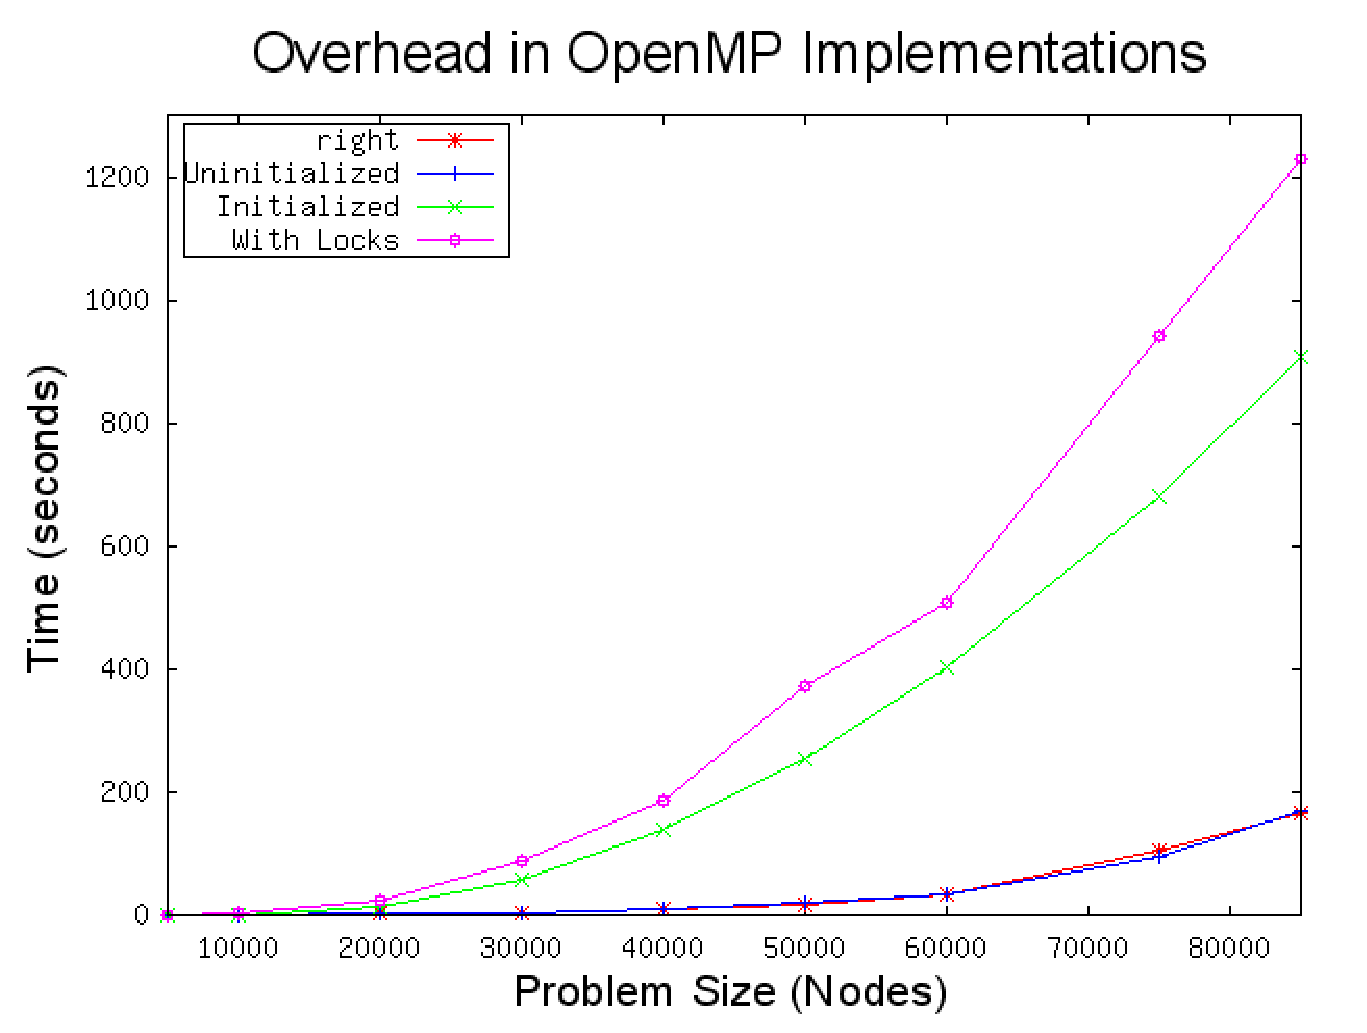
\includegraphics[scale=0.65]{figura1.eps}


\begin{tabular}{lrc}
Nombre & Edad & Clase \\
\hline
Jose & 24 & P \\
Juanito & 24 & P+\\
Carlos & 11 & Q-
\end{tabular}


\footnote{prueba3}

%++++++++++++++++++++++++++++++++++++++++++++++++++++++++++++++++++++++
\section{Entregable}
En la tarea habilitada para esta pr�ctica en el Aula Virtual, se subir� 
la direcci�n del repositorio \textit{github} donde se ha almacenado la pr�ctica. 
\subsection{}
Es importante entenderla.

%++++++++++++++++++++++++++++++++++++++++++++++++++++++++++++++++++++++
\section{Para saber m�s...}

Ampl�e el programa \textsf{Python} que ha desarrollado para que el n�mero de
subintervalos se pueda obtener tambi�n desde la l�nea de comandos.\cite{Libro de Python BULL} usado

\begin{thebibliography}{1}
\bibitem{python} Tutorial de Python. http://docs.python.org/2/tutorial/ 
\bibitem{python} Libro de Python BULL
\end{thebibliography}
\footnote{prueba4}

\end{document}
